\documentclass[%
% border=1pt
  border={0pt 0pt 0pt 0pt} % left bottom right top
]{standalone}% http://ctan.org/pkg/standalone

\usepackage{tikz}
\usepackage[defaultsans]{droidsans}
\renewcommand*\familydefault{\sfdefault} %% Only if the base font of the document is to be typewriter style
\usepackage[T1]{fontenc}

\begin{document}

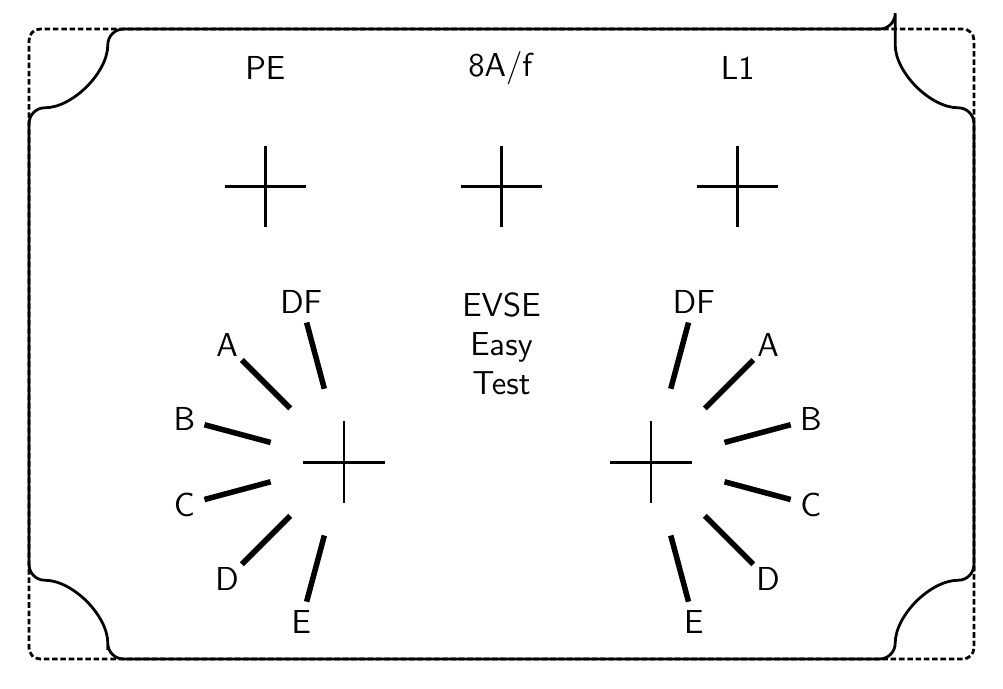
\begin{tikzpicture}[line cap=rect,line width=1pt]

% Bopla ET-215 frame
\draw[draw=black, dotted, rounded corners] (0,0) rectangle ++(120mm,80mm);
\draw [rounded corners=2mm] (0mm,70mm) arc[radius=10mm, start angle=-90, end angle=0] --
	(110mm,80mm) --
	(110mm,80mm) arc[radius=10mm, start angle=180, end angle=270] --
	(120mm,10mm) --
	(120mm,10mm) arc[radius=10mm, start angle=90, end angle=180] --
	(10mm,0mm) --
	(10mm,0mm) arc[radius=10mm, start angle=0, end angle=90] --
	cycle;

% Product name
\begin{scope}[shift={(60mm,40mm)}]
	\node[align=center, font=\large, text width=10mm] at (0:0mm)
	{\textsf\textbf{{EVSE Easy Test}}};
\end{scope}

% PE switch
\begin{scope}[shift={(30mm,60mm)}]
	\draw (0,5mm) -- (0,-5mm);
	\draw (5mm,0) -- (-5mm,0);
	\node[font=\large] at (90:15mm) {\textsf{PE}};
\end{scope}

% Fuse
\begin{scope}[shift={(60mm,60mm)}]
	\draw (0,5mm) -- (0,-5mm);
	\draw (5mm,0) -- (-5mm,0);
	\node[font=\large] at (90:15mm) {\textsf{8A/f}};
\end{scope}

% L1 LED
\begin{scope}[shift={(90mm,60mm)}]
	\draw (0,5mm) -- (0,-5mm);
	\draw (5mm,0) -- (-5mm,0);
	\node[font=\large] at (90:15mm) {\textsf{L1}};
\end{scope}


% State dial
\begin{scope}[shift={(79mm,25mm)}]
	%\draw (0,0) circle [radius=13.1mm];
	\draw (0,5mm) -- (0,-5mm);
	\draw (5mm,0) -- (-5mm,0);
	\foreach \angle/\label [count=\xi] in 
	{
		75/DF,45/A,15/B,-15/C,-45/D,-75/E
	}
	{
		\draw[line width=2pt] (\angle:10mm) -- (\angle:18mm);
		\node[font=\large] at (\angle:21mm) {\textsf{\label}};
	}
\end{scope}

% Max current dial
\begin{scope}[shift={(40mm,25mm)}]
	%\draw (0,0) circle [radius=13.1mm];
	\draw (0,5mm) -- (0,-5mm);
	\draw (5mm,0) -- (-5mm,0);
	\foreach \angle/\label [count=\xi] in
	{
		180-75/DF,180-45/A,180-15/B,180+15/C,180+45/D,180+75/E
	}
	{
		\draw[line width=2pt] (\angle:10mm) -- (\angle:18mm);
		\node[font=\large] at (\angle:21mm) {\textsf{\label}};
	}
\end{scope}



\end{tikzpicture}

\end{document}
